\documentclass[10pt,a4paper]{article}
\usepackage[margin=1.8cm]{geometry}
\usepackage{amsmath,amssymb}
\usepackage{graphicx}
\usepackage{booktabs}
\usepackage[font=small,labelfont=bf]{caption}
\usepackage{titlesec}
\titlespacing*{\section}{0pt}{8pt}{3pt}
\titleformat{\section}{\large\bfseries}{\thesection}{0.6em}{}
\setlength{\parskip}{3pt}
\setlength{\parindent}{0pt}
\pagestyle{empty}

\title{\vspace{-1.2cm}\textbf{Monte Carlo Integration of $\cos^2 x$ on $[0,2]$}\\[2pt]
\large MATH3602 -- Milestone 1\vspace{-0.3cm}}
\date{}
\begin{document}
\maketitle

\section{Method and analytic solution}
We estimate $I=\int_0^2\cos^2 x\,dx$. Using $\cos^2x=\tfrac12(1+\cos 2x)$,
\begin{equation}
I=\Big[\tfrac{x}{2}+\tfrac{\sin 2x}{4}\Big]_0^2 = 1+\tfrac{\sin 4}{4}\approx 0.810799 .
\end{equation}
The Monte Carlo estimator draws $x_i\sim U(a,b)$ and sets
$\hat I_n=\frac{b-a}{n}\sum_{i=1}^n f(x_i)$, which is unbiased. Its standard error is
\begin{equation}
\sigma_{\hat I}=\frac{(b-a)\,\sigma_f}{\sqrt n},\qquad
\hat\sigma_n=\frac{(b-a)\,s_f}{\sqrt n},
\end{equation}
where $\sigma_f^2=\mathrm{Var}[f(x)]$ and $s_f$ is its sample estimate, which is what
\texttt{monte\_carlo\_integral} returns as the error estimate. For this integrand, $\cos^4x=\tfrac38+\tfrac12\cos2x+\tfrac18\cos4x$ gives
$\sigma_f^2=\overline{\cos^4}-\overline{\cos^2}^{\,2}\approx0.1315$, so $\sigma_f\approx0.3626$ (confirmed numerically) and
\begin{equation}
\sigma_{\hat I}\approx \frac{0.725}{\sqrt n}.
\end{equation}
By the central limit theorem $\hat I_n$ is approximately Gaussian about $I$, so roughly 68\% of runs should land within $\hat\sigma_n$ of the true value and 95\% within $2\hat\sigma_n$.

\section{Monte Carlo results and error estimate}
A single run with $n=10^3$ (seed 3602) gives $\hat I=0.81277$ with estimated error $\hat\sigma=0.02265$; the actual error is $|\hat I-I|=0.0020$, about $0.09\hat\sigma$. A single run is not a test of the error estimate, so we also ran 500 independent repeats at each $n$ (Table~\ref{tab:res}) and compared the mean estimated error with the root-mean-square actual error. They agree to within a few percent for $n\ge100$ (at $n=10$ the sample variance is itself noisy). The estimator shows no significant bias.

Figure~\ref{fig:res}(a) shows one run at each of 1000 values of $n$ between $10$ and $10^6$. The actual error scatters around the estimate, with $68.6\%$ of runs inside $\hat\sigma_n$ and $95.7\%$ inside $2\hat\sigma_n$, matching the Gaussian expectation. A log--log fit of the actual error gives a slope of $-0.51$, consistent with the $n^{-1/2}$ law.

\begin{figure}[h]
\centering
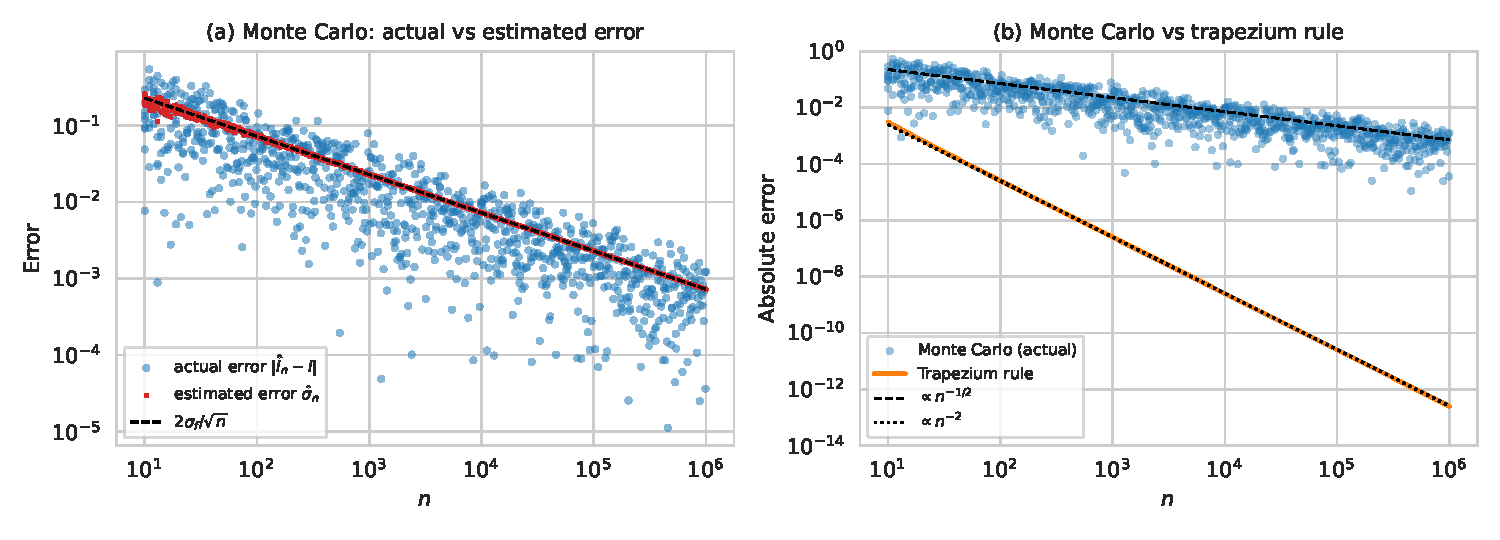
\includegraphics[width=\textwidth]{fig_results.pdf}
\caption{(a) Actual Monte Carlo error $|\hat I_n-I|$ (blue) and the estimated error $\hat\sigma_n$ (red) against the number of samples; the dashed line is $2\sigma_f/\sqrt n$. (b) Actual error of Monte Carlo and of the trapezium rule; the fitted trapezium slope is $-2.01$.}
\label{fig:res}
\end{figure}

\begin{table}[h]
\centering
\caption{Error against $n$. Monte Carlo columns use 500 repeats per $n$; the trapezium error is deterministic.}
\label{tab:res}
\begin{tabular}{rccc}
\toprule
$n$ & Mean est.\ error $\hat\sigma_n$ & RMS actual error (MC) & Trapezium error\\
\midrule
$10$     & $2.16\times10^{-1}$ & $2.28\times10^{-1}$ & $3.1\times10^{-3}$\\
$10^{2}$ & $7.21\times10^{-2}$ & $7.19\times10^{-2}$ & $2.6\times10^{-5}$\\
$10^{3}$ & $2.29\times10^{-2}$ & $2.29\times10^{-2}$ & $2.5\times10^{-7}$\\
$10^{4}$ & $7.25\times10^{-3}$ & $7.35\times10^{-3}$ & $2.5\times10^{-9}$\\
$10^{5}$ & $2.29\times10^{-3}$ & $2.22\times10^{-3}$ & $2.5\times10^{-11}$\\
$10^{6}$ & $7.25\times10^{-4}$ & $7.25\times10^{-4}$ & $2.5\times10^{-13}$\\
\bottomrule
\end{tabular}
\end{table}

\section{Extension: comparison with the trapezium rule}
The trapezium rule uses $n$ equally spaced points ($n-1$ panels, $h=(b-a)/(n-1)$). For a smooth integrand its error is
\begin{equation}
E_T\approx\frac{(b-a)^2}{12\,n^2}\,\big|f'(b)-f'(a)\big|=\frac{\sin 4}{3\,n^2}\approx\frac{0.252}{n^2},
\end{equation}
since $f'(x)=-\sin 2x$. The measured errors in Table~\ref{tab:res} follow this closely ($E_Tn^2\approx0.252$ for large $n$), and Figure~\ref{fig:res}(b) shows the $n^{-2}$ slope against Monte Carlo's $n^{-1/2}$. The gap is large: at $n=10^3$ the trapezium error is $\sim10^{5}$ times smaller. To match the trapezium error at only $n=100$ ($2.6\times10^{-5}$), Monte Carlo would need $(0.725/2.6\times10^{-5})^2\approx8\times10^{8}$ samples. The trapezium estimate is also deterministic, so its error curve is smooth rather than scattered, and in a quick timing test at $n=10^6$ it ran about three times faster (no random number generation). Simpson's rule, with error $O(h^4)$ for smooth integrands, would improve on this further (we did not run it).

\section{Conclusion}
The Monte Carlo estimate converges to the analytic value $1+\tfrac14\sin4\approx0.8108$, and the error estimate $(b-a)s_f/\sqrt n$ is reliable: it matches the RMS actual error and the expected 68\%/95\% coverage. However, for a smooth one-dimensional integral Monte Carlo is a poor choice, because its $n^{-1/2}$ convergence is far slower than the trapezium rule's $n^{-2}$ (or Simpson's $n^{-4}$). Monte Carlo pays off in high dimension $d$, where its rate stays $n^{-1/2}$ while grid-based quadrature degrades to roughly $n^{-2/d}$; the two break even near $d=4$.

\end{document}
